%!TEX root = ../../thesis.tex

%\section{Overview}

%Before discussing the software architecture in section~\ref{sec:software_architecture}, sections \ref{sec:rich_text_approaches} through \ref{sec:las_before_software_architecture} will discuss the apporaches, principles and goals for implementing this library without HTML editing APIs.

\section{Overview}
\label{sec:rich_text_approaches}

%When not using HTML editing APIs, the components and the bahavior of native text inputs must be imitated. There are various approaches to this.

%\subsection{Overlaying an element in editing mode} One way to 

This section will discuss the options to implement rich-text editing without relying (entirely) on HTML editing APIs and approaches to avoid their disadvantages and bugs. % and discuss the advantages and disadvantages of each method. % Diese Art zu schreiben sollte der Style der Arbeit sein.

\section{Native inputs, images and third-party plugins}

As discussed in \refsection{sec:alt_to_edit_apis}, native text inputs cannot be used for rich-text editing, using image elements has no benefits and many disadvantages and third-party plugins lack user adoption. For these reasons, none of these approaches will be considered.

\section{Enabling editing mode without using its API} One way to enable editing but avoid many bugs and browser inconsistencies, is to enable the editing mode on an element, but refrain from using \texttt{execCommand} to format the text. The latter could be implemented using the DOM core APIs. This would provide the user with all basic editing functions, i.e. a caret, text input, mouse interaction and clipboard capabilities---all of this would be taken care of by the browser.

This approach would solve the problem of buggy and inconsistent \texttt{execCommand} implementations but not the problems that arise with different browser behavior on the user's text input---for instance when entering a line break. If the markup is customly generated with JavaScript but the input would be handled by the browser's editing mode, the browser may not be able to work on the structures generated by JavaScript and break elements or simply get stuck. This was one of the reasons why Google decided to abandon editing APIs entirely\footnote{\url{http://googledrive.blogspot.fr/2010/05/whats-different-about-new-google-docs.html}, last checked on 07/21/2015}. It could be the source to many bugs and ultimately restrict the editors capabilities.

\section{Native text input imitation} 
\label{subsec:concept_native_imitation}

The only other option to allow the user to change the text on a website is by manually fetching the user's input and manipulating the DOM with JavaScript and DOM Level 1 APIs. However, this does not suffice to provide the experience of a text input. The following components, common to text editing, must also be accounted for:
% These components will be discussed hereinafter.

%, major browsers offer no way to place a caret

% Only native text input components and elements in editing mode
% ''ACE'' and ''CodeMirror'' demonstrate an effective way to imitate a text input. 

 %''ACE'' and ''CodeMirror'' demonstrate it is possible to imitate a text input by composing various DOM ele
\subsection{Caret} 

The caret is an essential part to text editing. Even if a user types on his or her keyboard, a caret must be seen on the screen to know where the input will be inserted. The caret also needs to be responsive to the user's interaction. In particular, the user must be able to click anywhere in the editable text and use the arrow keys to move it (possibly using modifier keys, which's behavior depends on the operating system used).

\subsection{Selection} 
The user must be able to draw a text selection using his or her mouse and change the selection using shift and the arrow keys. Most systems allow double clicks to select words and sometimes tripple clicks to select entire paragraphs. Other systems, for example OS X, allow holding the option key to draw are rectangular text selection, independent of line breaks.

\subsection{Context menu} The context menu is different in text inputs from other elements on a website. Most importantly, it offers an option to paste text, that is only available in native text inputs or elements in editing mode.

\subsection{Keyboard shortcuts} Text inputs usually allow keyboard shortcuts to format the text and to perform clipboard operations. Formatting the text is possible through DOM manipulation, pasting text however only works on text inputs or elements in editing mode. % is a challenge, since browsers do not offer arbitrary access to the clipboard for security reasons.

\subsection{Undo / Redo} Undo and redo are common functions of text processing and it may be frustrating to users if they were missing.

\subsection{Behavior} Rich-text editors (usually) share a certain behavior on user input. When writing a bulleted list, pressing the enter key usually creates another bullet point instead of inserting a new line. Pressing enter inside a heading will insert a new line. However pressing enter when the caret is located at the end of a heading commonly creates a new text paragraph after heading. %Other rules that need to be considered will be discussed in section [implementation].

\section{Approaches for imitating native components} 
\label{sec:approaches_for_imitating_native_components}

These components are natively available for text inputs across all browsers. Switching an element to editing mode enables these components too. That means users can click in a text to place a caret and move it with the keyboard's arrow keys. They can copy and paste text. The browser offers a native context menu that allows pasting on input elements as well as on element in editing mode. All major browsers implement a behavior for the users' input that is common for rich-text editing.

When not using editing APIs, all of this must be implemented with JavaScript. This requires a lot of trickery and many components must be imitated to make it \textit{seem} there is an input field, where there is none. The users must be convinced they are using a native input and must not notice they are not.

\begin{figure}[!htb]
\centering
\makebox[\textwidth]{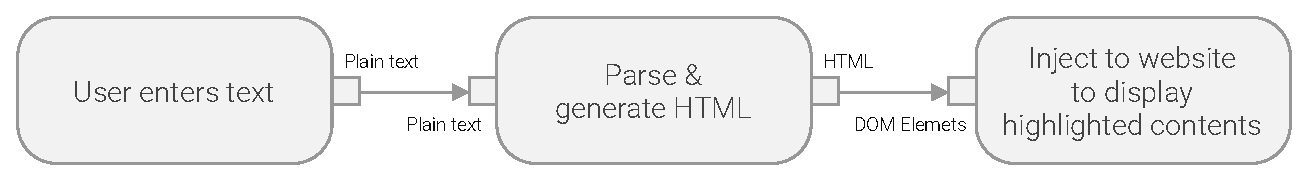
\includegraphics[width=\textwidth]{images/ace-codemirror-uml.eps}}
\caption{Rendering of highlighted source code in Ace and CodeMirror}
\label{fig:ace_rendering_uml}
\end{figure}


Web-based code editors like ''Ace''\footnote{\url{http://ace.c9.io/}, last checked on 08/22/2015} and ''CodeMirror'' demonstrate that this is possible. They display syntax-highlighted source code editable by the user. The user seemingly writes inside the highlighted text and is also presented with a caret as well as the above mentioned components. In reality, the content that the user sees is a ''regular'' part of the DOM---non-editable text, colored and formatted using HTML and CSS. When the user enters text, the input will be read with JavaScript. Based on the input Ace and CodeMirror generate HTML and add it to the editors contents, to show a properly syntax-highlighted representation (see figure~\ref{fig:ace_rendering_uml}). A \texttt{div} element that is styled to look like a caret is shown and moved with the user's keyboard and mouse input. The user's text input will be inserted at the according text offset. Amongst others, Ace and CodeMirror use DOM elements like \texttt{div}s to display a text selection and a \textit{hidden} \texttt{textarea} to fetch keyboard inputs, to recreate the behavior and capabilities of a native text input. % Google's document editor uses similar techniques too.

%In reality, the user's input will be read with JavaScript and the code he or she sees is HTML generated based on this input to display syntax-highlighted text. Other components, like the caret and even the selection \texttt{div} elements, styled and positioned to mimick their native counterparts. 

%All this creates the illusion of a native text input.

%Many of the techniques to mimick a native text input like this can be found in web-based code editors like ''ACE'' or ''CodeMirror''.

Using tricks and \textit{faking} elements or behavior is common in web front end development. This applies to JavaScript as well as to CSS. For instance, long before CSS3 has been developed, techniques have been discussed on how to implement rounded corners without actual browser support. Only years later, this has become a standard. This not only enables features long before the creators of browsers implement them, this \textit{feedback} by the community of web developers also influences future standards. Incorporating feedback is a core philosophy of the WHATWG, the original creators of HTML5.

%\section{Mimicking native components}

%As discussed in \refsection{sec:approaches_for_imitating_native_components}, the source code editors Ace and CodeMirror use various DOM elements to mimick a native text input while actually reading the user's input with JavaScript and displaying a custom ouput.

\section{Implementation}

The library implemented for this thesis uses similar techniques as Ace and CodeMirror to create a rich-text editor. The contents of the editor are represented by by a \code{div} element that contains the formatted text using HTML. The caret as a \code{div} element styled to mimic a native caret. The text selection is also displayed by using \code{div} elements that are styled accordingly. The keyboard and mouse input will be read with JavaScript and the contents of the editor will be changed accordingly using DOM Level 1 methods. The user's input will also be read to move the mimicked caret on the website with JavaScript. The specifics on the implementation of these components and how they interact will be discussed in \refchapter{ch:impl}.

% Ace, CodeMirror and Google's document editor share these concepts. 

%---and the other components discussed in \refsubsec{subsec:concept_native_imitation}---

% Google, unlike Ace and CodeMirror displays a custom context menu. 

\chapter{Software design}
\label{ch:concept_principles}

%\section{Overview}

%This chapter discusses principles chosen for its software design and the implementation of the library.

\begin{comment}
\section{Interaction with browser APIs}
\label{sec:interaction_with_browser_apis}

Interaction with the browser must be well chosen. In some cases browser interaction can cause bugs and slow down performance while in some cases it can increase performance. The library should conform these rules:

\begin{enumerate} 
\item Minimize interaction with the DOM
\item Minimize interaction with unstable APIs
\item Use browser APIs if it improves performance or structure
\end{enumerate}

DOM operations can trigger a browser reflow\footnote{\url{https://developers.google.com/speed/articles/reflow}, last checked on 07/19/2015} which slows down the browser's performance. For this reason DOM operations should be avoided where possible.

Some APIs like the browser's \texttt{Range} or \texttt{Selection} interface are useful but known to be unstable. Libraries like Rangy try to tackle this by shimming parts of the interfaces. This requires complex methods and it is hard to account for possibly unknown bugs in the browsers' APIs. Ultimately this will also affect the library's file size. Instead of trying to fix native APIs, only as little as possible should be used and pure JavaScript solutions should be implemented. Avoiding DOM operations and unstable APIs leads to a software architecture where the biggest part remains in its own business logic. % The only exception to this Anything that can be implemented in pure JavaScript and does not cost performance or memory \textit{should} be implemented in pure JavaScript using own methods and data structues. % Possibly unstable native APIs should only be used when it is inevitable.

Facebook defined a similar goal for the user interface library React. React implements virtual DOM, an internal representation of the actual DOM on which all operations should be performed, which in return does as little manipulation to the actual DOM as needed, to maximize performance. While the focus of this goal for this library is not solely performance, this part of it. However, there can be situations in which (even unstable) native browser methods may be faster than a JavaScript implementation. There can also be cases in which a pure JavaScript implementation would be much more complex and would be at the expense of having a simple code structure. It must be decided in each particular case to use native and possible unstable APIs or a pure JavaScript implementation while using as little interaction with the browser as possible is a maxim.

% The text flow for instance should be left to the browser.

%Improving means it should be more explicit in what it does. The \texttt{bold} command of \texttt{execCommand} will manipulate the DOM to format text bold. It does not state in what how. Simple etc, what I have stated at Disadvantages of offering user interface components.

\section{Markup} 
\label{sec:concept_markup}

As discussed in \refsubsec{subsec:noapi_dis_formatting}, the editor should be a ''good citizen'' in the ecosystem of other editors and should generate valid markup, expressing a formatting semantically correct with as few tags as possible. The algorithm for creating markup must be able to work on any markup parsable by the browser and in return must generate predictable, \textit{simple} markup itself. It must not inject markup required for the internal workings of the editor\footnote{Which is the case with FirePad and Google' document editor that inject markup necessary for the internal functions of the editors}.


% dom operations could also be cached
\end{comment}


\section{Implementation as pure library}

Most rich-text editors are implemented and distributed as user interface components. That means instead of only providing a library that offers methods to format the selected text and leaving the implementation of the user interface to the respective developer, most libraries are distributed as input fields with a default editor interface that is, at best, customizable.

This can be unfitting for many situations. The user interface of an editor highly depends on the software it will be integrated in. Within the software the interface may even vary depending on its specific purpose. For instance, a content management system may require an editor with a menubar offering many controls while a comment form on a blog requires only very little controls. Medium.com uses an interface that only shows controls when the user selects text and has no menubar at all. Assuming there are many implementations of editors that are functional, it can be argued, that choosing between editors is often really a choice of the desired user interface.

Customizing a user interface can be just as complex as writing an interface from scratch. The latter affords to add HTML elements and call JavaScript methods while both require styling. While adding HTML elements to a website is not a complex task, in a worst case scenario, it can be more complicated to customize an interface to specific needs than writing an interface from scratch and being able to define just the elements as they are required. 

As for the current state of the internet, web developers cannot easily implement a rich-text for themselves, they have to make a choice between pre-made solutions and customize them. Apart from the perspective of the user interface, integrating a fully featured editor into a software project can be invasive to the structure of the project.

For these reasons the library of this thesis will be implemented and distributed as a pure software library, offering developers an API to create a rich-text editor, rather than a fully implemented rich-text editor as a user interface component. 

%On a final note, until today, some rich-text editors use an iFrame to encapsulate the editor's contents and some don't. iFrame hat vor und nachteile. mit meiner library kann es jeder so machen, wie er/sie es will, weil es nur ne library ist.


\section{API}
\label{sec:api_design}
\label{sec:las_before_software_architecture}

%\subsection{Conformity with HTML Editing APIs}

The library should be capable of any method implemented by HTML editing APIs. However the API design can differ to improve they way it will be worked with. In particular the API and aims at providing a quick and simple way to create editable areas and connecting a user interfaces to it.

\subsection{API Design}

% It can be much more fitting for developers to include a library that handles all text-input and -formatting operations while only providing a powerful API, leaving the ui to the developer. 

% While it can be much more fitting for developers to use an API to implement an
The API of this library must be \textit{well-designed}. That means it must be simple, effective and fit the developers' needs. The methods it offers should be simple in the sense that they conceal possibly complex tasks with understandable high-level concepts. They should be effective and fit the developers' needs in the sense that the API should be designed so that any requirement to of the developers should be matched with as little effort as possible. The API should create a workflow for developers that allows them to do what they intend to do and is as easy to use and as plausible as possible. jQuery is an example of incorporating an API that comes close to these goals.

The library's API will have two basic use cases. On the one hand, web developers must be enabled to implement rich-text editors with it. On the other hand, the library should offer interfaces for enabling web developers to extend the library and add features.

\paragraph{Extension}

For extension, web developers should have precise access to as many components and functions of the library, providing as much freedom and options as possible. This will include low-level access to components while control and explicitness is more important than simplicity. 

All components of the library will be implemented as classes. To provide as much capabilities as possible to other developers, all classes of the library will be exposed in a designated namespace. The classes should conform the best practices of object-oriented programming to support developers in extending the library. The class design should not only consider the specific needs of the core library but also potential use cases for other developers.

For example, with a designated class to show and move a caret, multiple carets can be instantiated for an extension that allows real-time collaboration with multiple users. All available classes will be discussed in chapter \refchapter{ch:impl}.

\paragraph{Editor implementation}

For web developers implementing an editor, the API should be designed to offer methods for the most common tasks related to rich-text editing to allow fast and easy integration in a website. This should be high-level methods as compared to methods required for extending the library. Simplicity is more important than precise control over low-level behavior. For implementing a rich-text editor the exposed methods should cover

\begin{enumerate}
\item Formatting and removing formats
\item Insertion
\item Deletion
\item Controlling the caret
\item Controlling the text selection
\item Controlling the clipboard
\item Controlling settings
\item Undo / redo commands
\end{enumerate}

\noindent jQuery demonstrates an effective and simple approach to API design, conforming the principles as discussed above. In jQuery all methods remain in a flat hierarchy within the root of a jQuery collection. Any method that is not a getter allows chaining and most methods are overloaded to allow passing various kinds of parameters, to determine what the function should do. Following these and the above-mentioned principles, the components listed above can be expressed in 11 functions:

\begin{lstlisting}[language=JavaScript, caption=API for implementing a rich-text editor, label=lst:rich_text_api]
editor.caret([options]);
editor.selection([options]);
editor.insert([options]);
editor.format([options]);
editor.remove([options]);
editor.settings([options]);
editor.copy();
editor.cut();
editor.paste();
editor.undo();
editor.redo();
\end{lstlisting}

\noindent The functions in lines 1 through 6 can take various overloaded parameters to determine the specific action. The selection command, for instance, can be called with two numbers to draw a selection from one character offset to another. To draw a selection from characters 10 to 20 \code{editor.selection(10, 20)} can be called. The function can also be called without passing any parameters to read the selection. \code{editor.selection()} will return the currently selected contents. A full API description can be found in tables \ref{table:instance_api_caret_command} through \ref{table:instance_api_options_command}.

%Applied to Type, this means

%As discussed in \refsubsec{subsec:flawed_api}, the HTML editing APIs, while being high-level and simple, still lack control and can be improved in that sense while still being simplified. As proposed in \refsubsec{subsec:adv_flawed_api}, to simplify the API and to increase control, all 17 formatting commands will be replaced with a single \code{format} method that accepts an \code{htmlString} compatible to jQuery.

%\noindent This will even account for cases where it is necessary to differenciate between an \code{i} element and an \code{em} element for semantical reasons.

\subsection{Handling use cases}
\label{subsec:api_design_handling_use_cases}

We can call programmers extending the library ''developers of the library'' and programmers using the library to implement editors ''users of the library''. To account for both use cases and maintain a clear software architecture as well as a separation of concerns, all classes that provide functionality to the library must remain in a designated namespace which the library has access to. Developers of the library have access to the namespace and can utilize any of its classes to extend its functions.

\begin{figure}[!htb]
\centering
\makebox[\textwidth]{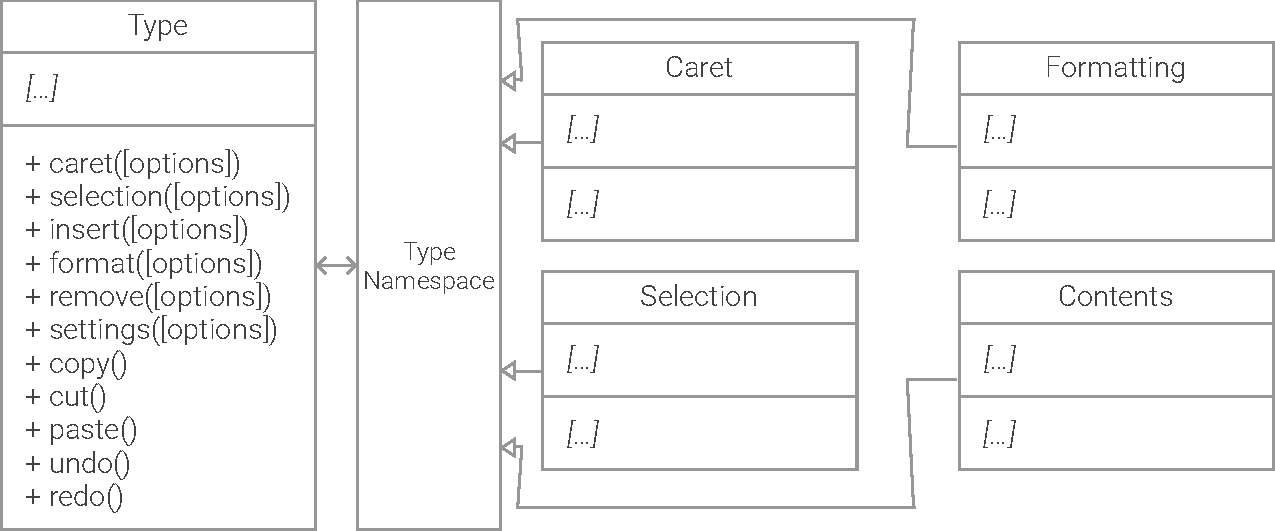
\includegraphics[width=\textwidth]{images/concept-sep-use-cases.pdf}}
\caption{Diagram of the Type library and its internally used classes (excerpt)}
\label{fig:type_uml_excerpt}
\end{figure}

The classes within the namespace will be used by a globally accessible class called ''Type'' which is the entry point for the users of the library to implement rich-text editors. The Type class provides an API with all of the above-mentioned methods and uses the classes inside the namespace for their implementation. It must be instantiated and be passed an element on the website (for example a \code{div} element) which it will then use as its ''editor contents''. The users of the library can build an interface for this editable element and use the instance's API to edit its rich-text contents.

%Users of the library can access the globally available ''Type'' class that provides all methods for the implementation of a rich-text editor.

%The library itself will be exposed as a class to the global namespace with the name ''Type''. It can be instantiated and then provides an own API---high-level methods---for implementing a rich-text editor.

%Ursprünglich API und Codestruktur an window.execCommand orientiert, das ist aber doof.
%Bessere (weil präzisere) API mit mehr Möglichkeiten als der contentEditable scheiss
%für Programmierer und für 2 anwendungsfälle:
%einen editor bauen
%type mit plugins erweitern
%für beides gibt es die passenden Funktionen, das eine einfach und schlau, das andere präzise
%Deswegen werden auch alle Module, alle Klassen exponiert aber es gibt eine eigene API nach jQuery konzept
%Type kommt mit bestimmten Kernmodulen die fuer Textbearbeitung essenziell sind. Aber an dieser Stelle laesst sich Type um weitere Module anhand einer KOnvention (erweitern des Type Objekts) erweitern.
%Ursprünglich API und Codestruktur an window.execCommand orientiert, das ist aber doof.

%The library shall give other developers as much freedom as possible, meaning other developer should use the library as they see it fit and not the other way around, should try to conform the needs of the library.


\section{Distribution}

The library will be distributed as a single JavaScript file. Extensions by third-party developers will each be distributed as independent and separate (JavaScript) files. By exposing Type and its classes as discussed in section \refsection{sec:api_design} they can be accessed from other files. This provides a modular ''plug and play'' system for distributing and loading extensions. To improve loading times, web developers can concatenate Type and its extensions to a single file in a web project.



%\textit{Ace, CodeMirror and Google's document editor shre similar concepts for imitating a native text input. For the caret, each of the editors create a \texttt{div} element, style it to make it look like a caret and move it when the user clicks in the text or uses his or her arrow keys. Each editor also uses \texttt{div} elements to display a text selection, styled to imitate the user's operating system's native selections.} %In fact, there is hardly no alternative way

%\textit{The concept to use HTML elements for the visible components of text editing is inevitable. Anything that can be seen on a website must exist in the DOM. The only deviation to this approach would be to resort a \texttt{canvas} element, as discussed above. The apporach to use HTML elements will be used for the implementation of this editor.}

%\textit{Hacks are a necessity for an editor like this. The following sections will discuss each part of the editor and describe ideas, techniques and hacks that can be used for an effective implementation. In prior, we will discuss goals and principles that these techniques should be oriented towards as well as restrictions of browsers these techniqes must adapt to. BEHANDLE DIE THEMEN GAR NICHT SO} % worst sentence ever



\chapter{Architecture}
\label{sec:impl_architecture}

%Modulbasiert?
%Erweiterbarkeit
%Es gibt ein Basisobjekt, das ist die Type "Klasse".
%Darin werden dann die anderen Klassen geschrieben "Type.Caret", "Type.Selection", "Type.Range", ...
%Das hat den Vorteil dass das ganze ge-name-spaced ist, so dass ich keine Konflikte mit Systemnamen habe (Range) (und auch nicht mit anderen Bibliotheken)
%Effektiv gibt es eine (flache) Baumstruktur und so mit Ordnung. Für bestimmte Klassen, "Type.Event.Input", "Type.Input.Filter.X" geht es tiefer.
%Der zweite Grund ist, dass ich somit alle Klassen die ich geschrieben habe für Entwickler sichtbar bereit stelle und nicht implizit und versteckt über irgend nen Quatsch.

%Auch angedacht so wie der CKEditor (?) die komplette funktionalität als Plugins zu schreiben. Im Besten Fall

\section{Model--view--controller}
\label{sec:mvc_architecture}

Model--view--controller (MVC) is a common approach for implementing user interfaces and it can be applied to user interface components too. While this approach can provide clear responsibilities, the problem is that most components, like the caret or the selection, serve a clear atomic purpose and would need to be broken apart into model, view and controller parts themselves, making the architecture fuzzy and complex instead of simplifying it.

Following the MVC architecture, the contents of the editor (the text) can be represented in a model (holding the text data and allowing methods to be performed on) and be rendered with a view (displaying the text in the browser). In contrast to the beforementioned components, this would be a a very clean model for implementing the editor's contents. It is even imaginable to implement multiple renderers in the view layer, turning the editor from rich-text into a Markdown editor, for instance.

Unfortunately, this approach would make the contents of the editor only editable through the API of the ''Type'' library. If any other script on a website would change its contents, the library's renderer would overwrite the changes with the next rendering the data of the internal model. As discussed in \refsection{sec:api_design}, the library shall leave as much freedom as possible to the developers. This would create a bottleneck and restrict other developers. For this reason, the MVC architecture will not be used.

%As discussed in \refsection{sec:api_design}, the library shall leave as much freedom as possible to the developers. In and MVC system like this, the contents of the editor could only be changed though the API, since arbitrarily modifying the HTML of the editor's contents would change the view, but not the model. This would create an artificial bottleneck, which cannot be desired.

%The biggest advantage of this approach would be that an abstract view layer could not only render rich-text as HTML, but also as Markdown or in the Open Document Format (ODF). Atom, Spotify or Wunderlist show that web technologies find their way into desktop. Writing to custom formats 
%While especially the latter is not useful in a browser environment


%Ursprünglich ein MVC konzept geplant mit einem Document Model und verschiedenen Renderern, aber über den haufen geworfen.

%\subsection{Modular programming}

\section{Modular and object-oriented programming}
\label{subsec:modular_and_oop}

jQuery and CKEditor demonstrate a software architecture in which a base object, which is exposed to other developers as the library, provides an environment to extend its functionality, but does not offer many methods itself\footnote{CKEditor provides a framework for implementing components for it, but does not offer any rich-text functionality in its core. jQuery provides low-level utility methods for JavaScript.}. The actual functionality of both libraries is implemented through extensions while the libraries are usually bundled with a set of ''core extensions'' that provide basic features. CKEditor makes use of modular programming techniques by implementing a major part of its editor as plugins that communicate via strictly defined interfaces. jQuery established a paradigm calling any extension a ''plugin'' but instead of using strictly defined interfaces, developers are encouraged to add arbitrary methods to jQuery's base object, which can then be directly accessed. Extending a base object has many advantages:

\begin{enumerate}
\item It provides a namespace for the library
\item It provides a structure for extensions to access each other
\item It approaches modular programming and strong decoupling
\end{enumerate}

Strict modular programming could create a system in which other developers can exchange any component easily to improve performance or enrich functionality. The disadvantage this approach would be that the need for well-defined interfaces can diminish flexibility. Formalizing interfaces would create complex structures and could make it harder for other developers to contribute to the library instead of inviting them. jQuery uses another approach and encourages arbitrary extensions. jQuery's approach demonstrates that this flexibility, in practice, can withstand possible conflicts. In turn, the low barrier for extending jQuery has spawned a rich collection of extensions and a big community of developers. While jQuery technically allows to be extended with complex libraries, it is designed to be extended with simple methods. It is difficult to establish complex interactions between extensions.

% However, the biggest factor in coupling the components would still be that components reference each other, not the underlying structure. 


\subsection{Constructor Pattern \& modularized structure}
\label{subsec:const_pat_and_modules}

To close the gap between CKEditor's modular programming approach and jQuery's simple extension paradigms, object-oriented programming (OOP) can be used. JavaScript does not offer classes and classical inheritance, however the same functionality can be achieved using the constructor pattern and prototypal inheritance (see \refsection{sec:oop_class}). Functions following the constructor pattern are often called classes or pseudo-classes. Hereinafter the term classes will be used.

%\begin{lstlisting}[language=JavaScript, caption=Type instantiation, label=lst:type_instantiation]
%// Defines the class and its contructor 
%function Foo() {
%  this.instanceVariable = "bar";
%};
%
%// Defines a method for the class
%Foo.prototype.baz = function() {
%  alert(this.instanceVariable);
%};
%
%// Instantiates the class
%var myFooInstance = new Foo();
%
%// alerts "bar"
%myFooInstance.baz();
%\end{lstlisting}

%In JavaScript the \code{new} operator can be used to create instances of \code{Function} objects. Based on prototypical inheritance each instance will share the same methods and attributes of the function's \code{prototype} property, but can still own instance-specific variables and functions by assiging them to the instance object. 


% maybe explain constructor pattern

% \subsection{Modularized structure} 

%As discussed in \refsubsec{subsec:api_design_handling_use_cases}, the base class will be called ''Type'' and be globally accessible. It will create a namespace

As discussed in \refsubsec{subsec:api_design_handling_use_cases}, the base class will be globally accessible with the name ''Type''. It will provide the namespace for classes that extend the library and implement its functionality. A set of core extensions will provide all components needed for a rich-text editor. The ''Type'' base class can be instantiated and will be the entry point for \textit{users} of the library (see \refsubsec{subsec:api_design_handling_use_cases}) to implement a rich-text editor. Like CKEditor and jQuery, will implement as little functionality as possible itself. The implementation of the base class as well as the interaction of its extensions will be discussed in detail in chapter \refchapter{ch:impl}. Implementing the library's extensions as classes has many benefits:

%For this library a base class will provide the namespace to be extended with other classes implementing the functionality of this library. A set of core extensions provide all components needed for a rich-text editor. The base class will also provide a constructor that will be the library's entry point for \textit{users} of the library (see \refsubsec{subsec:api_design_handling_use_cases}) to implement a rich-text editor, but, like CKEditor and jQuery, will implement as little functionality as possible itself. The implementation of the base class as well as the architecture and interaction of its extensions will be discussed in detail in chapter \refchapter{ch:impl}. Implementing the library's extensions as classes has many benefits:

\begin{enumerate}
\item As compared to CKEditor and modular programming, strictly defined interfaces are not a necessity. This can improve flexibility and lower the barrier for other developers to contribute. % Auf Nachteile eingehen?
\item As compared to jQuery, classes can have complex interfaces, which allows rich functionality and possibilities in interaction.
\item Classes are a proven concept for encapsulating functionality and data, protecting access and structuring code as well as making it readable.
\item Through JavaScript's prototypical inheritance, the class can be instantiated as often as desired, but will only be allocated once in the browser's memory. Thereby the performance will be improved. Instance variables still allow to reuse a class in different contexts with different inherent data. %Die instanzvariablem sind meistens nur Pointer auf Instanzen anderer Klassen % * Das ganze ist dadurch sehr schlank
\end{enumerate}

%As an alternative apporach, the module pattern can be used, which would also allow namespacing, encapsulation and protected access, but would make an implementation much more complicated and be much less readable.

%namespace vorteile = keine namenskonflikte

% and implement as many components as possible as plugins. In its core, the library could create an environment to allow plugins to register and interact with each other. This would 

